Le bain initial correspond à un bain oxyde avec une masse initiale de 10 T, une température initiale de 2900 K et une composition de 0.77 UO$_2$ - 0.12 Zr - 0.11 ZrO$_2$ (ratio molaire $R_{U/Zr}$ = 1.3 et degré d'oxydation du zirconium $C_{Zr}$ = 30 \%). La puissance résiduelle constante $\dot{\mathcal{Q}} = 200$ MW est portée par l'espèce uranium U. Une condition adiabatique est imposée sur la couche d'acier liquide hors équilibre du bain (FE.), sinon, pour le bain sous la croûte, la température d'interface pour la couche supérieure est la température de fusion de la croûte. Les propriétés physiques des couches du bain sont calculés en fonction de la composition et de la température de la couche par un code externe. Enfin, les caractéristiques utiles des différentes couches du bain sont détaillées dans le tableau~\ref{tab:caracteristiques_couches_bain}, en particulier les températures de \textit{liquidus} $T^{fus}$ ainsi que les corrélations de flux de chaleur utilisées pour le calcul des puissances latérales $\phi S$ (voir~\cite{Bonnet1999} ou~\cite{Tourniaire2009a} pour plus de détails sur les corrélations).
\begin{table}
	\centering
	\begin{tabular}{ccc} 
	\hline
	Couche & $T^{fus}$ (K) & Corrélation latérale\\
	\hline
	Acier liquide (FE.) & 1800 & ChurchillAndChu\\
	Métal léger (LM.) & 1800 & ChurchillAndChu\\
	Oxyde (OX.) & 3000 & BaliDownWard\\
	Métal lourd (HM.) & 1800 & BaliDownWard\\
	\hline
	\end{tabular}	
	\caption{Configuration initiale du bain de corium pour le test.} 
	\label{tab:caracteristiques_couches_bain}
\end{table}

Différentes coulées d'acier liquide à différents instants du calcul permettent de reproduire des stratifications du bain d'intêret pour les calculs accidents graves. En particulier, ces coulées ont été calculées en fonction du seuil d'inversion de stratification du bain (correspondant à quantité d'acier dans la bain permettant le passage d'un état d'équilibre thermochimique composé d'une couche de métaux lourds en dessous d'une couche d'oxydes vers un équilibre composé d'une couche d'oxydes en dessous d'une couche de métaux légers). Les caractéristiques de ces coulées (temps de début et de fin, masse, température et composition) sont détaillés dans le tableau~\ref{tab:coulees_acier}. 
\begin{table}
	\centering
	\begin{tabular}{ccccc} 
	\hline
	$t_{\text{début}}$ (s) &  $t_{\text{arrêt}}$ (s) & Débit (kg/s) & T (K) & Composition\\
	\hline
	15 000 & 15 200 & 5 & 1805 & 0.687 Fe - 0.208 Cr - 0.106 Ni\\
	30 000 & 30 200 & 8 & 1805 & 0.687 Fe - 0.208 Cr - 0.106 Ni\\
	\hline
	\end{tabular}	
	\caption{Les différentes coulées d'acier liquide imposées pour le test.} 
	\label{tab:coulees_acier}
\end{table}
Un temps suffisament long entre chacune de ces coulées est imposé pour permettre au bain d'atteindre un état quasi-stationnaire de thermique et de thermochimie. Les différentes configurations quasi-stationnaires du bain obtenues (OX. puis HM./OX. puis OX./LM.) sont décrites dans la figure~\ref{fig:stratifications_bains}.
\begin{figure}
\centering
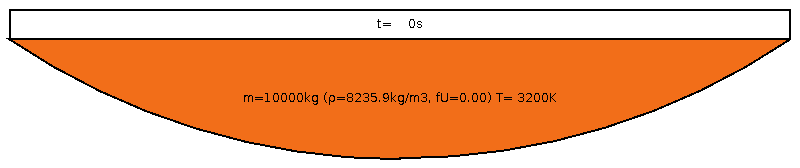
\includegraphics[width=0.85\textwidth, keepaspectratio=true]{Figures/coriumPool_t=00000.png}\\
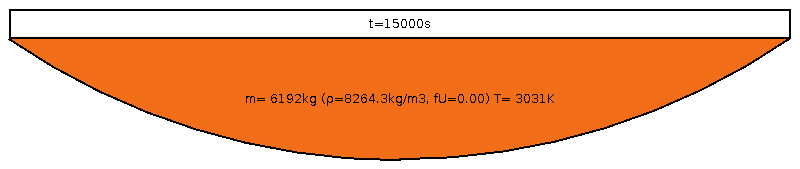
\includegraphics[width=0.85\textwidth, keepaspectratio=true]{Figures/coriumPool_t=15000.png}\\
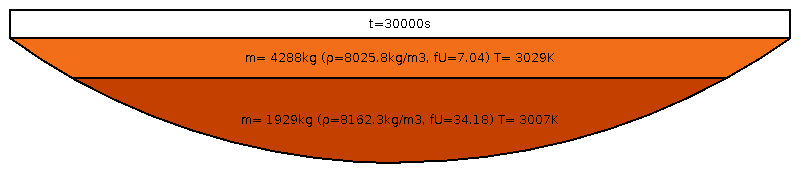
\includegraphics[width=0.85\textwidth, keepaspectratio=true]{Figures/coriumPool_t=30000.png}\\
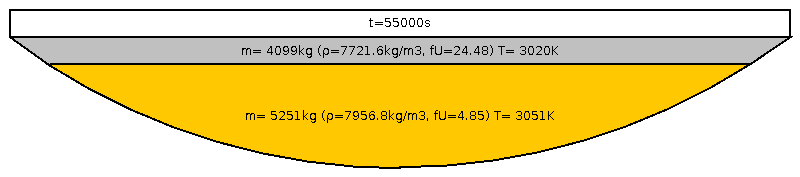
\includegraphics[width=0.85\textwidth, keepaspectratio=true]{Figures/coriumPool_t=55000.png}
\caption{La configuration initiale et les différentes stratifications quasi-stationnaires du bain de corium en fond de cuve atteintes lors du test : \textcolor{yellow!75!black}{\textbf{OX.}} à t=15 000 s puis \textbf{HM.}/\textcolor{yellow!75!black}{\textbf{OX.}} à t=30 000 s puis \textcolor{yellow!75!black}{\textbf{OX.}}/\textcolor{gray}{\textbf{LM.}} à t=55 000 s.}
\label{fig:stratifications_bains}
\end{figure}

Enfin, la croûte est divisée, tout au long du calcul, en 20 mailles. La puissance résiduelle constante $\dot{\mathcal{Q}} = 200$ MW dans la croûte est portée par l'espèce uranium U. Le résidu d'apparition de la croûte est de 5 mm. Une température constante et uniforme de 1800 K est imposée sur les parois exterieures de la croûte (seul le couplage entre le modèle de bain de corium et le modèle de croûte sont testés ici).

Durant les différentes étapes du transitoire, de la masse est échangée entre le bain de corium et sa croûte par solidification du bain ou fusion de la croûte. À chaque macro pas de temps du calcul et en fin de calcul, \emph{on vérifie bien la conservation de la masse globale du système}.

De la même manière, de l'énergie est échangée entre le bain de corium et la croûte et \emph{on vérifie la conservation globale de l'énergie du système}. La figure~\ref{fig:thermal_balance} donne les différentes puissances d'intêret du bain de corium et de la croûte au cours du transitoire.
\begin{figure}
\centering
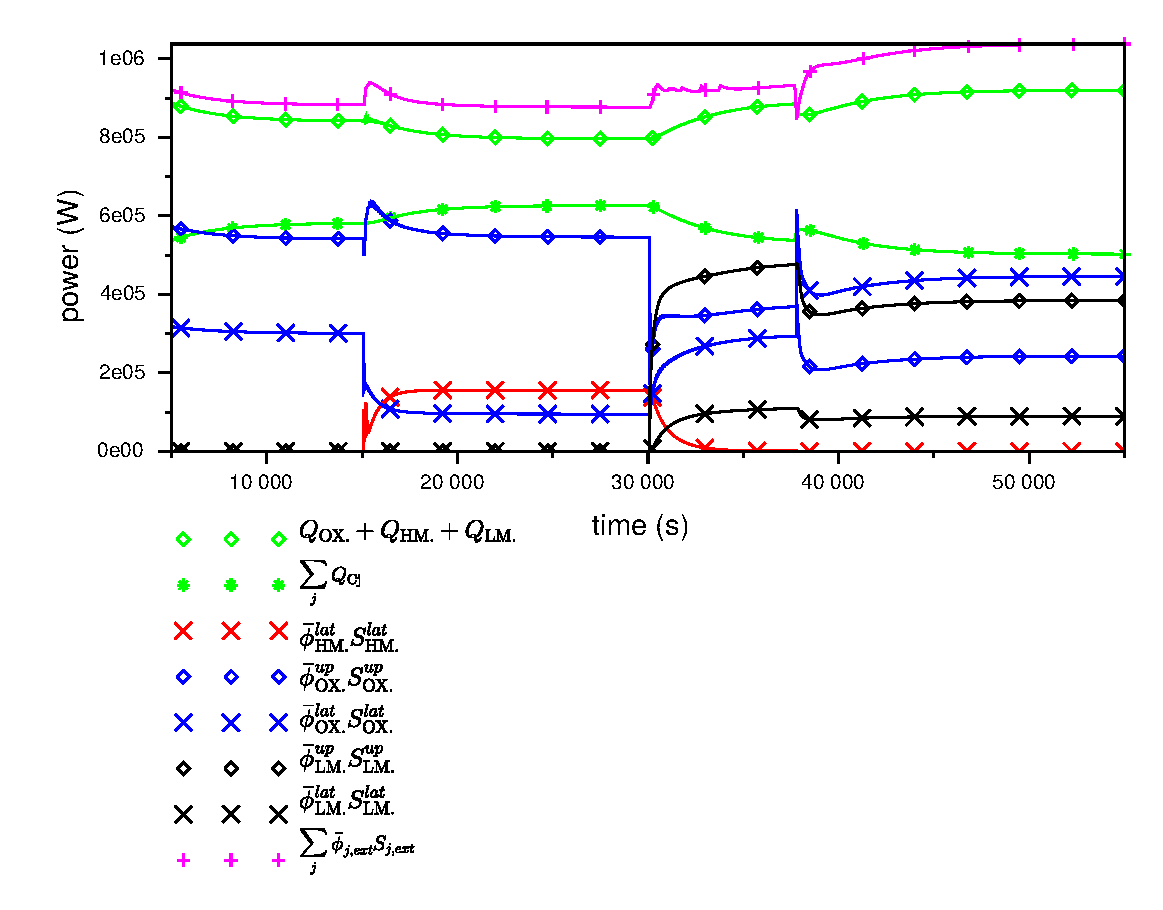
\includegraphics[width=\textwidth, keepaspectratio=true]{Figures/thermal_balance.eps}\\
\caption{Puissances d'intêret du système bain de corium et croûte.}
\label{fig:thermal_balance}
\end{figure}
En particulier, les puissances évacuées par les surfaces latérales des différentes couches du bain 
\begin{equation*}
\bar{\phi}^{lat}_\textrm{HM.}S^{lat}_\textrm{HM.},\,\bar{\phi}^{lat}_\textrm{OX.}S^{lat}_\textrm{OX.},\,\bar{\phi}^{lat}_\textrm{LM.}S^{lat}_\textrm{LM.}
\end{equation*}
et par sa surface supérieure 
\begin{equation*}
\bar{\phi}^{up}_\textrm{OX.}S^{up}_\textrm{OX.}\,\text{pourt <= 16 000 s  puis}\,\bar{\phi}^{up}_\textrm{LM.}S^{up}_\textrm{LM.},
\end{equation*}
la somme des puissances résiduelles des couches du bain $Q_\textrm{OX.}+Q_\textrm{HM.}+Q_\textrm{LM.}$ ainsi que la somme des puissances résiduelles $Q_{C_j}$ des mailles $C_j$ de la croûte, et enfin la somme des puissances $\bar{\phi}_{j,ext}S_{j,ext}$ évacuées par la surface extérieure $\gamma_{ext}$ des mailles $C_j$ de la croûte. La conservation de l'énergie peut être vérifiée graphiquement dans la figure~\ref{fig:thermal_balance} aux trois états quasi-stationnaires atteints. Par exemple, pour t=15 000 s, on a :
\begin{equation}
\bar{\phi}^{up}_\textrm{OX.}S^{up}_\textrm{OX.} + \bar{\phi}_{j,ext}S_{j,ext} = Q_\textrm{OX.} + \sum_j Q_{C_j}.
\end{equation}

Durant le transitoire, les mailles de la croûte passent dans les différents états décrits dans la section~\ref{sect:thermique} (solidification, conduction et fusion). En particulier, pour la première partie du transitoire pour t $\leq$ 15 000 s, la croûte se solidifie jusqu'à atteindre un état quasi-stationnaire de solidification (voir figure~\ref{fig:croutes_1}).  
\begin{figure}
\centering
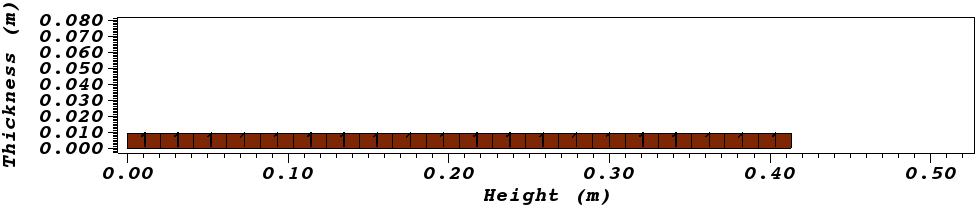
\includegraphics[width=\textwidth, keepaspectratio=true]{Figures/croute_0.png}\\
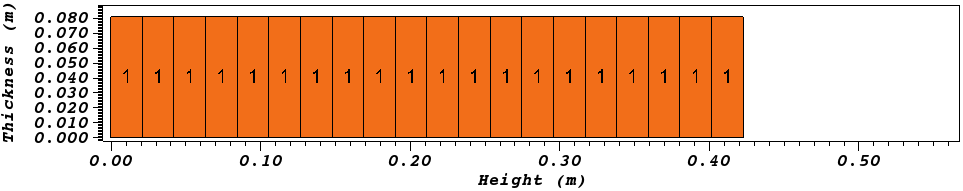
\includegraphics[width=\textwidth, keepaspectratio=true]{Figures/croute_1.png}
\caption{Croûte à t = 100 s (en haut) et à t = 15 000 s (en bas). \textit{L'indice dans la maille $C_j$ donne la couche de bain en face de celle-ci : 0 $\Leftrightarrow$ HM., 1 $\Leftrightarrow$ OX., 0 $\Leftrightarrow$ LM., 3 $\Leftrightarrow$ FE., -1 $\Leftrightarrow$ pas de contact avec le bain}.}
\label{fig:croutes_1}
\end{figure}

Lors de la seconde partie du transitoire, la couche de métal lourd apparaît suite à une coulée d'acier liquide (voir tableau~\ref{tab:coulees_acier}). La figure~\ref{fig:croutes_2} donne les différents états de la croûte durant ce transitoire.
\begin{figure}
\centering
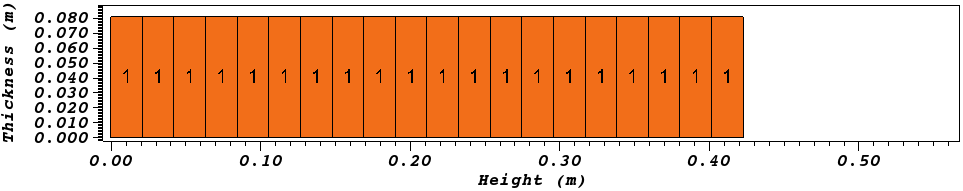
\includegraphics[width=\textwidth, keepaspectratio=true]{Figures/croute_1.png}\\
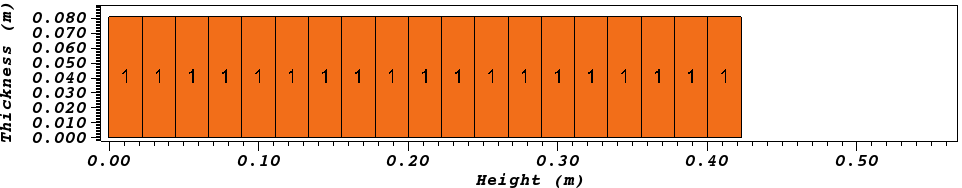
\includegraphics[width=\textwidth, keepaspectratio=true]{Figures/croute_2.png}\\
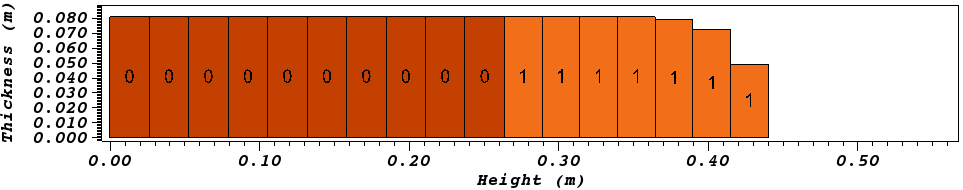
\includegraphics[width=\textwidth, keepaspectratio=true]{Figures/croute_3.png}\\
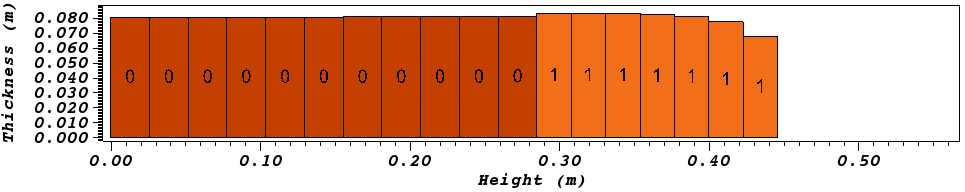
\includegraphics[width=\textwidth, keepaspectratio=true]{Figures/croute_4.png}\\
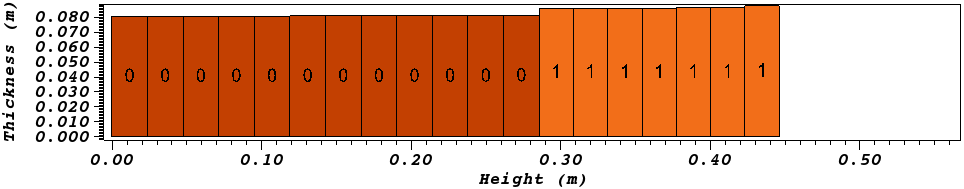
\includegraphics[width=\textwidth, keepaspectratio=true]{Figures/croute_5.png}\\
\caption{De haut en bas, croûte à t = 15 000 s, t=15 100 s, t=16 000 s, t=18 000 s, t=30 000 s (état quasi-stationnaire du bain HM./OX.). \textit{L'indice dans la maille $C_j$ donne la couche de bain en face de celle-ci : 0 $\Leftrightarrow$ HM., 1 $\Leftrightarrow$ OX., 0 $\Leftrightarrow$ LM., 3 $\Leftrightarrow$ FE., -1 $\Leftrightarrow$ pas de contact avec le bain}.}
\label{fig:croutes_2}
\end{figure}
Entre t=15 000 s et t=15 100 s, une maille de croûte apparaît en face d'une couche d'acier liquide (à une hauteur h > 0.42 m) provenant de la coulée et le maillage de la croûte oxyde passe de 20 mailles (à t=15 000s) à 19 mailles (à t=15 100s). Cette maille de croûte acier apparaît avec une épaisseur initiale de 5 mm mais fond presque instantanément et disparaît. Ensuite, la couche de métal lourd s'épaissit et le volume du bain augmente du fait des propriétés physiques différentes des couches HM. et OX.. Par conséquent, une croûte oxyde apparaît au fur et à mesure (voir les figures à t=16 000 s et t=18 000 s). À t=30 000 s, la thermochimie et la thermique du bain se sont stabilisées et la croûte n'évolue plus : on retrouve bien les profils plats de flux projetés sur les mailles de la croûte. 

